\documentclass{article}

\usepackage[a4paper,margin=2.5cm]{geometry}
\usepackage{graphicx}
\usepackage{amsmath}
\usepackage{amssymb}
\usepackage{listings}
\usepackage{amsthm}
\usepackage{hyperref}
\usepackage{amsfonts}
\usepackage{parskip}

\graphicspath{images}

\newcommand{\code}[1]{\texttt{#1}}

\title{Object Oriented Programming Report}
\author{Giorgio Grigolo}
\date{Semester 1, 2022}

\begin{document}

\maketitle
\begin{abstract}
This report is a summary of the Object Oriented Programming course.
\end{abstract}

\tableofcontents

\newpage

\section{Minesweeper --- A C++ Implementation}

\subsection{Introduction}
Minesweeper is a logic puzzle video game genre generally played on personal
computers. The game features a grid of clickable squares, with hidden ``mines''
scattered throughout the board. The objective is to clear the board without
detonating any mines, with help from clues about the number of neighboring
mines in each field.
In this section (\thesection), we will implement Minesweeper with the help of
ncurses\footnote{Ncurses is a programming library providing an application with a 
terminal-independent screen-painting and keyboard-handling facility in a
text-mode environment.} and C++.

The game is played on a board of tiles, each of which is either a mine or
empty. The player is initially presented with a board of tiles, and
must use logic to deduce the locations of the mines. The player can click on a
tile to reveal it. If the tile is a mine, the player loses. If the tile is
empty, the tile will be revealed, and if it has no neighboring mines, all of
its neighboring tiles will be revealed as well. If the tile has neighboring
mines, the number of neighboring mines will be displayed on the tile. If the player
marks all of the mines, the player wins.


\subsection{Implementation}

\subsubsection{UML}

\vspace{9em}
\begin{figure}[h]
\centering
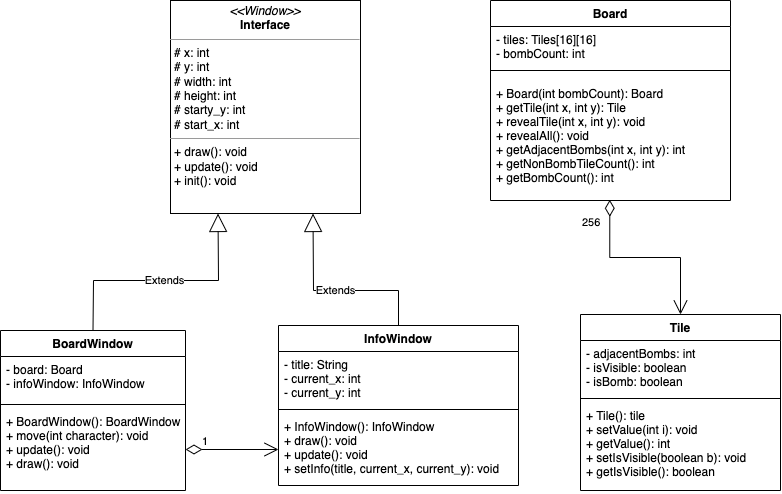
\includegraphics[width=0.9\textwidth]{images/minesweeper.png}
\caption{Minesweeper UML Diagram}
\end{figure}

\newpage

\subsection{Design Choices}

The user interface, to be preferably displayed on a full screen terminal, is
usable through the traditional `\code{wasd}' keys, or the vim\footnote{Vim is a free and open-source, screen-based text editor.}-oriented `\code{hjkl}' keys, and the `\code{Space}'
key to reveal a tile.

The user interface uses the ncurses library. Being by far the most
difficult part of this program that I had to implement, it was the one that required most of 
my attention and time. Even though it originated in the form of a C library, I have created
an abstract handler class \code{Window}, in such a way that I thought would best fit the
needs of this program. The window class is inherited by the two windows that are shown
to the user: the \code{BoardWindow} and the \code{InfoWindow}.

The \code{BoardWindow} will tile by tile, get the properties of the tile, and
display them accordingly; either hidden or revealed. In case of the latter, the number 
of adjacent mines will be shown, in an appropriate color. The \code{InfoWindow} will display the current selected coordinates, mostly for debugging
purposes. When the game is over be it won or lost, it will display the final message respectively.

Of course, each window type update and draw methods are different, as they have different
properties to display. Whilst inheriting a common interface, they are still
different classes.

As for the board, it made sense for it to act as a storage for the tiles, as well as a 
handler for the different tile states. One could say that the \code{Board} is a list-like data structure, 
with utility functions modifying the internal state for every atomic object inside of it, the \code{Tile}.

A \code{Tile} is just a POCO (a plain old C++ object), which means that the class only contains privated class variables, together with their public 
getters and setters, thus making it encapsulated and low-coupled.


\subsection{Testing}

The game, being simple in nature, is easy to test. I have tested
the \code{Board} class by creating a board with a given number of mines, and
then checking if the number of mines is correct. I have also tested the
\code{Board} class by checking if the number of adjacent mines is correct.

This was done through manual inspection, together with a hidden keybind set to `\code{C}' that would reveal all the tiles.
A second debug keybind was set to `\code{B}' which would turn the currently selected tile into a mine, 
to see that the adjacent mines were correctly calculated.

The win condition was tested by generating a board with all mines except for one tile, and clicking on it
 which is known to us given the \code{revealAll} function, which is called when `\code{C}' is pressed.

 A lot of care has been put in such a way that on quitting, (keybind: `\code{Q}'), the windows are destroyed 
 through the pipeline provided by ncurses \code{endwin()}, as to reduce as many memory leaks as possible.

\subsection{Critical Evaluation and Limitations}

The game is fully functional, and it is playable. It is also easy to use, and
it is very intuitive. The game was developed with scalability in mind, and one can set 
the board size and the number of mines in the \code{Board} class.

However, the game is not perfect, and it has some limitations. One of these is the fact that
user interface is not resizable, and it will look unplayable on a terminal smaller than
29x102 characters.

Also, since the mines are randomly generated, the game can be lost in the first move, which is not the way 
the original minesweeper works. The original minesweeper would randomly seed the board mine position randomization process
 after the first move, in such a way that your first move is never a mine.

 \newpage

\section{Village War Game --- A Java Implementation}

\subsection{Introduction}
This gam


\end{document}
